\documentclass[11pt]{article}

\usepackage[T1]{fontenc}
\usepackage{lmodern}
\usepackage{microtype}
\usepackage[margin=0.82in,headheight=15pt]{geometry}
\usepackage{mathtools,amssymb,amsthm}
\usepackage{xcolor}
\usepackage[most]{tcolorbox}
\usepackage{enumitem}
\usepackage{fancyhdr}
\usepackage{hyperref}
\usepackage{tikz}
\usetikzlibrary{patterns,positioning}

\definecolor{ink}{HTML}{172230}
\definecolor{navy}{HTML}{243B53}
\definecolor{indigo}{HTML}{4C51BF}
\definecolor{mint}{HTML}{2A9D8F}
\definecolor{amber}{HTML}{E9A23B}
\definecolor{coral}{HTML}{E76F51}
\definecolor{mist}{HTML}{EDF6F5}
\definecolor{paper}{HTML}{FCFBF7}
\definecolor{muted}{HTML}{617080}

\pagecolor{paper}
\color{ink}
\hypersetup{
  colorlinks=true,
  linkcolor=mint,
  urlcolor=coral,
  pdfauthor={Igor Rivin},
  pdftitle={Probability Problem Set 1: The Geometry of Events}
}

\setlength{\parindent}{0pt}
\setlength{\parskip}{4pt}
\setlist[enumerate,1]{label=\textbf{\arabic*.},leftmargin=*,itemsep=10pt,topsep=6pt}
\setlist[enumerate,2]{label=(\alph*),leftmargin=1.75em,itemsep=4pt,topsep=4pt}
\setlist[itemize]{leftmargin=1.5em,itemsep=2pt,topsep=3pt}

\newcommand{\points}[1]{\hfill\textcolor{coral}{\small\bfseries[#1 points]}}
\newcommand{\edition}{\ifsolutions Worked Solutions\else Student Handout\fi}
\newcommand{\blank}[1]{\ifsolutions\else\vspace{#1}\fi}

\pagestyle{fancy}
\fancyhf{}
\fancyhead[L]{\small\color{muted}Problem Set 1}
\fancyhead[R]{\small\color{muted}Chance, Data, and Decisions}
\fancyfoot[C]{\color{mint}\thepage}
\renewcommand{\headrulewidth}{0.3pt}

\newtcolorbox{overviewbox}{
  enhanced,breakable,colback=mist,colframe=mint,boxrule=.8pt,arc=2mm,
  left=4mm,right=4mm,top=2.5mm,bottom=2.5mm,
  borderline west={3pt}{0pt}{mint}
}

\newtcolorbox{instructornote}{
  enhanced,breakable,colback=amber!8,colframe=amber,boxrule=.7pt,arc=2mm,
  title={Instructor note},fonttitle=\bfseries\color{navy}
}

\NewDocumentEnvironment{solution}{+b}{%
  \ifsolutions
    \begin{tcolorbox}[
      enhanced,breakable,colback=white,colframe=mint!55,boxrule=.55pt,arc=1mm,
      left=3mm,right=3mm,top=2mm,bottom=2mm,
      title={\small\bfseries Solution},title after break={\small\bfseries Solution (continued)},
      fonttitle=\small\bfseries,coltitle=navy]
      \small #1
    \end{tcolorbox}
  \fi
}{}

\newcommand{\ThreeVennNumbered}{%
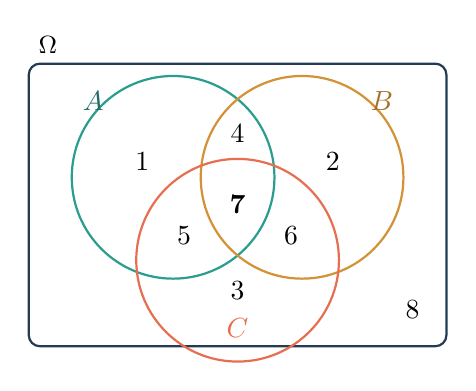
\begin{tikzpicture}[scale=.78]
  \draw[rounded corners,thick,navy] (-3.4,-2.25) rectangle (3.4,2.35);
  \draw[thick,mint] (-1.05,.50) circle (1.65);
  \draw[thick,amber!90!black] (1.05,.50) circle (1.65);
  \draw[thick,coral] (0,-.85) circle (1.65);
  \node[font=\bfseries,text=mint!70!black] at (-2.35,1.75) {$A$};
  \node[font=\bfseries,text=amber!70!black] at (2.35,1.75) {$B$};
  \node[font=\bfseries,text=coral] at (0,-1.95) {$C$};
  \node at (-1.55,.75) {1};
  \node at (1.55,.75) {2};
  \node at (0,-1.35) {3};
  \node at (0,1.22) {4};
  \node at (-.87,-.45) {5};
  \node at (.87,-.45) {6};
  \node[font=\bfseries] at (0,.05) {7};
  \node at (2.85,-1.65) {8};
  \node[above right,font=\small] at (-3.4,2.35) {$\Omega$};
\end{tikzpicture}}

\newcommand{\VennDifference}{%
\begin{tikzpicture}[scale=.68]
  \draw[rounded corners,thick,navy] (-2.8,-1.55) rectangle (2.8,1.75);
  \ifsolutions
    \fill[mint!42] (-.75,.05) circle (1.15);
    \begin{scope}\clip (-.75,.05) circle (1.15);\fill[paper] (.75,.05) circle (1.15);\end{scope}
  \fi
  \draw[thick,mint] (-.75,.05) circle (1.15);
  \draw[thick,amber!90!black] (.75,.05) circle (1.15);
  \node at (-1.15,.1) {$A$}; \node at (1.15,.1) {$B$};
  \node[above right,font=\small] at (-2.8,1.75) {$\Omega$};
\end{tikzpicture}}

\newcommand{\VennOutsideUnion}{%
\begin{tikzpicture}[scale=.68]
  \ifsolutions\fill[amber!30,rounded corners] (-2.8,-1.55) rectangle (2.8,1.75);\fi
  \draw[rounded corners,thick,navy] (-2.8,-1.55) rectangle (2.8,1.75);
  \ifsolutions
    \fill[paper] (-.75,.05) circle (1.15);
    \fill[paper] (.75,.05) circle (1.15);
  \fi
  \draw[thick,mint] (-.75,.05) circle (1.15);
  \draw[thick,amber!90!black] (.75,.05) circle (1.15);
  \node at (-1.15,.1) {$A$}; \node at (1.15,.1) {$B$};
  \node[above right,font=\small] at (-2.8,1.75) {$\Omega$};
\end{tikzpicture}}

\newcommand{\VennIntersectionOrC}{%
\begin{tikzpicture}[scale=.68]
  \draw[rounded corners,thick,navy] (-2.8,-1.9) rectangle (2.8,2.05);
  \ifsolutions
    \fill[coral!34] (0,-.55) circle (1.15);
    \begin{scope}\clip (-.75,.25) circle (1.15);\fill[mint!38] (.75,.25) circle (1.15);\end{scope}
  \fi
  \draw[thick,mint] (-.75,.25) circle (1.15);
  \draw[thick,amber!90!black] (.75,.25) circle (1.15);
  \draw[thick,coral] (0,-.55) circle (1.15);
  \node at (-1.35,.75) {$A$}; \node at (1.35,.75) {$B$}; \node at (0,-1.35) {$C$};
  \node[above right,font=\small] at (-2.8,2.05) {$\Omega$};
\end{tikzpicture}}

\begin{document}

\begin{tcolorbox}[
  enhanced,colback=paper,colframe=navy,boxrule=1.1pt,arc=2mm,
  left=5mm,right=5mm,top=3.5mm,bottom=3.5mm,
  borderline west={5pt}{0pt}{mint}]
  {\Large\bfseries\color{navy}Problem Set 1: The Geometry of Events}
  \hfill{\bfseries\color{mint}\edition}\\[3pt]
  {\large Sets, Venn diagrams, De Morgan's laws, and inclusion--exclusion}\\[4pt]
  {\small\color{muted}80 points + 10 optional challenge points}
  \ifsolutions\else
    \\[7pt]\textbf{Name:}\ \rule{0.46\linewidth}{0.4pt}\hfill
    \textbf{Due:}\ \rule{0.21\linewidth}{0.4pt}
  \fi
\end{tcolorbox}

\begin{overviewbox}
\textbf{Purpose.} Sets are the grammar in which probability will be written.
This assignment develops fluency in translating among words, symbols, Venn
diagrams, and counts. Give reasons for your answers: a diagram may support an
argument, but it does not replace one when a proof is requested.

\textbf{Notation.} All complements are taken relative to the stated universe
$\Omega$. The symbol $|A|$ denotes the number of elements in a finite set $A$.
The word ``or'' is inclusive unless explicitly stated otherwise.
\end{overviewbox}

\ifsolutions
\begin{instructornote}
The core assignment is Problems 1--8. Problem 3 checks visual translation;
Problems 4 and 5 move from pictures to inclusion--exclusion; Problems 6--8
provide a gentle transition from examples to proof. The challenge can be
assigned even if divisibility has not been discussed formally.
\end{instructornote}
\fi

\section*{I. Sets in symbols and pictures}

\begin{enumerate}
\item \textbf{Membership and operations.} \points{10}
Let
\[
  \Omega=\{1,2,3,4,5,6,7,8,9,10,11,12\},\quad
  A=\{2,4,6,8,10,12\},\quad
  B=\{2,3,5,7,11\}.
\]
List the elements of each set.
\begin{enumerate}
  \item $A\cap B$
  \item $A\cup B$
  \item $A^c$
  \item $A\setminus B$
  \item $(A\cup B)^c$
\end{enumerate}
\begin{solution}
The sets $A$ and $B$ are, respectively, the even elements and the prime
elements of $\Omega$. Directly checking membership gives
\begin{align*}
 A\cap B&=\{2\},\\
 A\cup B&=\{2,3,4,5,6,7,8,10,11,12\},\\
 A^c&=\{1,3,5,7,9,11\},\\
 A\setminus B&=\{4,6,8,10,12\},\\
 (A\cup B)^c&=\{1,9\}.
\end{align*}
Notice that $2$ belongs to both $A$ and $B$, while $1$ and $9$ belong to
neither.
\end{solution}

\item \textbf{Negating carefully: De Morgan's laws.} \points{10}
Let $A,B\subseteq\Omega$.
\begin{enumerate}
  \item Translate $(A\cup B)^c=A^c\cap B^c$ into an English sentence.
  \item Prove the identity in part (a) by showing that an arbitrary element
  $x\in\Omega$ belongs to the left side exactly when it belongs to the right.
  \item State the other De Morgan law and prove it in the same way.
\end{enumerate}
\begin{solution}
\begin{enumerate}
  \item ``Being in neither $A$ nor $B$ is the same as being outside $A$ and
  outside $B$.'' Equivalently, ``not ($A$ or $B$)'' means ``not $A$ and not $B$.''
  \item For any $x\in\Omega$,
  \begin{align*}
  x\in(A\cup B)^c
  &\iff x\notin A\cup B\\
  &\iff (x\notin A)\text{ and }(x\notin B)\\
  &\iff (x\in A^c)\text{ and }(x\in B^c)\\
  &\iff x\in A^c\cap B^c.
  \end{align*}
  Since this holds for every $x$, the sets are equal.
  \item The other law is $(A\cap B)^c=A^c\cup B^c$. Indeed,
  \begin{align*}
  x\in(A\cap B)^c
  &\iff x\notin A\cap B\\
  &\iff (x\notin A)\text{ or }(x\notin B)\\
  &\iff (x\in A^c)\text{ or }(x\in B^c)\\
  &\iff x\in A^c\cup B^c.
  \end{align*}
\end{enumerate}
\end{solution}

\item \textbf{Reading and shading Venn diagrams.} \points{12}

In the numbered diagram below, each number labels one of the eight disjoint
regions determined by $A$, $B$, and $C$.
\begin{center}\ThreeVennNumbered\end{center}
\begin{enumerate}
  \item Give the region number(s) belonging to each set:
  \[
  A\cap B\cap C,\qquad A\setminus(B\cup C),\qquad
  (A\cup B)^c,\qquad (A\cap B)\setminus C.
  \]
  \item Shade the requested set in each diagram.
\end{enumerate}
\begin{center}
\begin{tabular}{ccc}
\VennDifference & \VennOutsideUnion & \VennIntersectionOrC\\[-2pt]
$A\setminus B$ & $(A\cup B)^c$ & $(A\cap B)\cup C$
\end{tabular}
\end{center}
\begin{solution}
For part (a), the region lists are
\[
\begin{array}{c|c}
\text{set}&\text{regions}\\ \hline
A\cap B\cap C&7\\
A\setminus(B\cup C)&1\\
(A\cup B)^c&3,8\\
(A\cap B)\setminus C&4
\end{array}
\]
The diagrams above show the required shading. In the third diagram, all of
$C$ is shaded, together with the lens $A\cap B$ (including any overlap that
the lens already has with $C$).
\end{solution}
\end{enumerate}

\section*{II. Counting with overlaps}

\begin{enumerate}[resume]
\item \textbf{Two-set inclusion--exclusion.} \points{10}
Among 120 students, 68 study calculus, 54 study programming, and 31 study both.
Assume every student is among the 120 being surveyed.
\begin{enumerate}
  \item How many study calculus or programming (or both)?
  \item How many study exactly one of the two subjects?
  \item How many study neither subject?
  \item Explain briefly why simply adding $68+54$ gives the wrong answer to part (a).
\end{enumerate}
\begin{solution}
Let $C$ be the calculus set and $P$ the programming set.
\begin{enumerate}
  \item Inclusion--exclusion gives
  \[
    |C\cup P|=|C|+|P|-|C\cap P|=68+54-31=91.
  \]
  \item There are $68-31=37$ calculus-only students and $54-31=23$
  programming-only students, hence $37+23=60$ who study exactly one subject.
  \item The number studying neither is $120-91=29$.
  \item In $68+54$, each of the 31 students in the overlap is counted twice.
  Subtracting the overlap once makes each such student count exactly once.
\end{enumerate}
\end{solution}

\item \textbf{A three-set survey.} \points{14}
At a university with 200 surveyed students, let $M,C,E$ denote the students
taking mathematics, computing, and economics. Suppose
\[
\begin{gathered}
|M|=105,\quad |C|=90,\quad |E|=75,\\
|M\cap C|=50,\quad |M\cap E|=40,\quad |C\cap E|=35,\\
|M\cap C\cap E|=20.
\end{gathered}
\]
The pairwise intersection counts include students taking all three subjects.
\begin{enumerate}
  \item Determine the number in each of the eight regions of a three-set Venn diagram.
  \item How many students take at least one of the three subjects?
  \item How many take exactly one? Exactly two? All three? None?
  \item Check that your four answers in part (c) add to 200.
\end{enumerate}
\begin{solution}
Start from the center. The triple intersection contains 20 students. Thus
the pair-only regions have sizes
\[
  MC\text{ only}=50-20=30,\quad
  ME\text{ only}=40-20=20,\quad
  CE\text{ only}=35-20=15.
\]
Subtracting all overlap regions from each set gives
\[
  M\text{ only}=105-30-20-20=35,
\]
\[
  C\text{ only}=90-30-15-20=25,
  \qquad E\text{ only}=75-20-15-20=20.
\]
Therefore the union has size
\[
  35+25+20+30+20+15+20=165,
\]
so 35 students lie outside all three sets. Equivalently, three-set
inclusion--exclusion gives
\[
|M\cup C\cup E|=105+90+75-50-40-35+20=165.
\]
Exactly one subject: $35+25+20=80$. Exactly two: $30+20+15=65$.
All three: 20. None: 35. Finally,
\[
  80+65+20+35=200,
\]
as required.
\end{solution}

\item \textbf{Difference distributes over union.} \points{10}
\begin{enumerate}
  \item Use De Morgan's law and the identity $A\setminus B=A\cap B^c$ to
  simplify $A\setminus(B\cup C)$.
  \item Prove directly, by following an arbitrary element $x$, that
  \[
    A\setminus(B\cup C)=(A\setminus B)\cap(A\setminus C).
  \]
  \item Explain the identity in one ordinary English sentence.
\end{enumerate}
\begin{solution}
\begin{enumerate}
  \item We calculate
  \[
  A\setminus(B\cup C)
  =A\cap(B\cup C)^c
  =A\cap(B^c\cap C^c)
  =(A\cap B^c)\cap(A\cap C^c),
  \]
  where the final equality uses associativity and the fact that repeating
  $A$ changes nothing. This is $(A\setminus B)\cap(A\setminus C)$.
  \item For any $x\in\Omega$,
  \begin{align*}
  x\in A\setminus(B\cup C)
  &\iff x\in A,\ x\notin B,\text{ and }x\notin C\\
  &\iff x\in A\setminus B\text{ and }x\in A\setminus C\\
  &\iff x\in(A\setminus B)\cap(A\setminus C).
  \end{align*}
  \item The elements of $A$ that are in neither $B$ nor $C$ are precisely
  those that remain after removing both $B$ and $C$ from $A$.
\end{enumerate}
\end{solution}
\end{enumerate}

\section*{III. From diagrams to arguments}

\begin{enumerate}[resume]
\item \textbf{Cancellation can fail for sets.} \points{6}
The equation $a+c=b+c$ implies $a=b$ for numbers. Decide whether each proposed
analogue for sets is true. Prove it if it is true; give a concrete
counterexample if it is false.
\begin{enumerate}
  \item If $A\cup C=B\cup C$, then $A=B$.
  \item If both $A\cup C=B\cup C$ and $A\cap C=B\cap C$, then $A=B$.
\end{enumerate}
\begin{solution}
\begin{enumerate}
  \item This is false. Take $A=\{1\}$, $B=\{2\}$, and $C=\{1,2\}$.
  Then $A\cup C=C=B\cup C$, but $A\ne B$.
  \item This is true. Let $x\in A$. If $x\in C$, then
  $x\in A\cap C=B\cap C$, so $x\in B$. If $x\notin C$, then
  $x\in A\cup C=B\cup C$; because $x\notin C$, we must have $x\in B$.
  Thus $A\subseteq B$. The same argument with $A$ and $B$ interchanged gives
  $B\subseteq A$, hence $A=B$.
\end{enumerate}
\end{solution}

\item \textbf{Why three-set inclusion--exclusion works.} \points{8}
For finite sets $A,B,C$, prove
\[
|A\cup B\cup C|=|A|+|B|+|C|
-|A\cap B|-|A\cap C|-|B\cap C|+|A\cap B\cap C|.
\]
Do this by choosing one element $x$ and checking its total contribution to
the right-hand side when $x$ belongs to exactly zero, one, two, or three of
the sets.
\begin{solution}
Consider a fixed element $x$. If $x$ belongs to none of the sets, it
contributes 0 to every term. If it belongs to exactly one set, it appears once
among $|A|,|B|,|C|$ and nowhere else, so its contribution is 1. If it belongs
to exactly two sets, it is added twice among the single-set terms and
subtracted once in the corresponding pairwise intersection, contributing
$2-1=1$. If it belongs to all three sets, it is added three times, subtracted
three times, and added once in the triple intersection, contributing
$3-3+1=1$. Thus every element of the union is counted exactly once and every
element outside the union is counted zero times. The two sides are equal.
\end{solution}
\end{enumerate}

\section*{Optional challenge}

\begin{enumerate}[resume]
\item \textbf{Inclusion--exclusion among the integers.} \points{10 optional}
How many integers from 1 through 500 are divisible by at least one of
$4$, $6$, or $9$? How many are divisible by none of them? Show how every
term in your inclusion--exclusion calculation arises.
\begin{solution}
Let $A_d$ be the set of integers from 1 through 500 divisible by $d$. Then
$|A_d|=\lfloor500/d\rfloor$. Intersections correspond to least common
multiples:
\[
\begin{array}{c|ccccccc}
\text{set}&A_4&A_6&A_9&A_4\cap A_6&A_4\cap A_9&A_6\cap A_9&A_4\cap A_6\cap A_9\\ \hline
\text{divisor}&4&6&9&12&36&18&36\\
\text{size}&125&83&55&41&13&27&13
\end{array}
\]
Therefore
\[
|A_4\cup A_6\cup A_9|
=125+83+55-41-13-27+13=195.
\]
The other $500-195=305$ integers are divisible by none of $4,6,9$.
\end{solution}
\end{enumerate}

\vfill
\begin{center}
\small\color{muted}
Before submitting: check complements against $\Omega$, include overlaps when
you write ``or,'' and make every inclusion--exclusion correction visible.
\end{center}

\end{document}
